% Rozdziały zaczynają się od "chapter"
\chapter{Wstęp}
% Praca podzielona na mniejsze pliki włączane za pomocą input
\chapter{Wstęp}

Świat jest odwzorowywany przez programy komputerowe za pomocą modeli.
Zawierają one~uproszczoną reprezentację rzeczywistości, a logika programu
umożliwia wykonywanie obliczeń na podstawie modelu, jego modyfikację, lub
utrwalenie i udostępnienie do wglądu innym osobom.
Modele te mogą być prezentowane użytkownikowi na wiele sposobów. Jednym z~nich
jest reprezentacja graficzna w~formie diagramu. Taka metoda reprezentacji
pozwala użytkownikowi na łatwiejsze zrozumienie modelu
oraz jego modyfikację, w porównaniu do~formatu tekstowego, ponieważ jest
wizualna i przestrzenna, a więc jest naturalniejszą formą dla mózgu człowieka.

Przykładem modeli z reprezentacją graficzną, które są zrozumiałe zarówno dla
człowieka, jak i maszyny, oraz
przydają się podczas wytwarzania oprogramowania, są modele korzystające
z~\emphgls{UML}~\cite{wikipedia-uml}. Przedstawiają
one strukturę klas w programie oraz zależności między klasami. Na ich podstawie
czytelnik może wysokopoziomowo zapoznać się~ze strukturą programu, a
odpowiednie narzędzia pozwolą wygenerować kod klas w danym języku
programowania, który może służyć jako początek do późniejszego rozwoju
aplikacji. Przykładowy model \emphgls{UML} został przedstawiony na
rysunku~\ref{rys:przykladowy-model-uml}.

\begin{figure}[!ht]
	\centering
	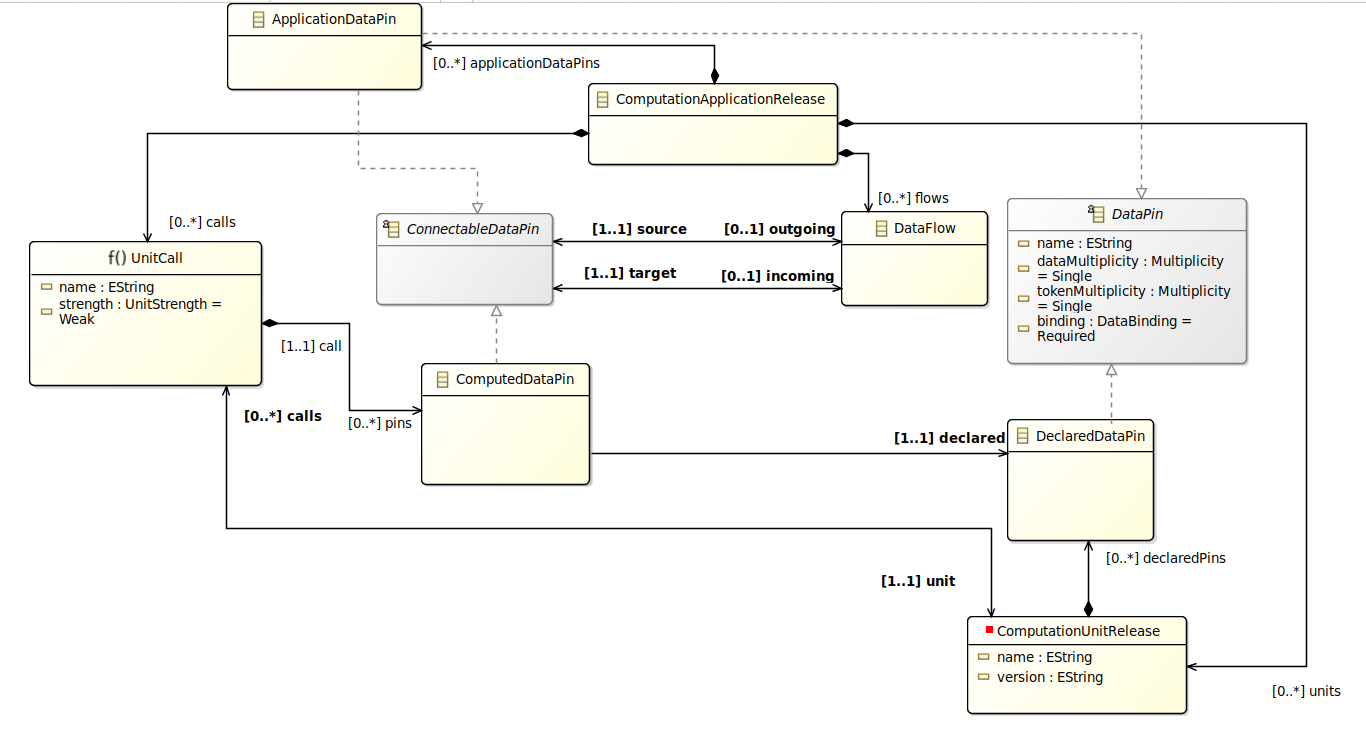
\includegraphics[width=0.9\linewidth]{./images/example-uml-model.png}
	\caption{Przykładowy model
		\emphgls{UML}}\label{rys:przykladowy-model-uml}
\end{figure}

\emphgls{UML} jest przykładem uniwersalnego języka do opisu modeli klas
programu.
Nie jest on~związany z żadną konkretną tematyką klas i pozwala na modelowanie
programów o~różnym zastosowaniu i przeznaczeniu. Istnieją także języki do opisu
modeli ściślej związanych z~konkretną dziedziną, czyli \emphgls{DSL}. Takie
języki
są zazwyczaj mniejsze i mniej skomplikowane od języków uniwersalnych, a także
mają dokładniejszą semantykę (znaczenie elementów modelu). Potrafią więc one
odwzorować rzeczywistość w~sposób bardziej kompletny i zawrzeć więcej
szczegółów.

Strukturę samego modelu opisuje metamodel. Jest to model, który definiuje jakie
są~możliwe typy elementów modelu, jakie mają atrybuty, jak są połączone ze
sobą (składnia języka modelowania). Sam metamodel może być opisany na przykład
w języku \emphgls{UML} lub podobnym
bazowanym na nim, który będzie umożliwiał wprowadzenie większej liczby
szczegółów. Taki metamodel często należy uzupełnić o zasady semantyczne ---
informacje o znaczeniu elementów, które nie mogą być zapisane w strukturze
metamodelu.
Przykładową informacją semantyczną w metamodelu języka \emphgls{UML} może być
znaczenie relacji kompozycji i wynikających z niej dozwolonych i niedozwolonych
ustawień elementów.

\BalticLSC{} jest platformą do obliczeń rozproszonych wykonywaną z
inicjatywy
\emph{INTERREG Regionu Morza Bałtyckiego Unit Europejskiej}. Platforma ta
pozwala
wykonać obliczenia wykorzystując dostępne jednostki obliczeniowe. Aplikacje
obliczeniowe definiowane są w postaci diagramów przedstawiających przepływ
danych między jednostkami obliczeniowymi. Przykład diagramu opisującego
aplikację
obliczeniową został przedstawiony na
rysunku~\ref{rys:przykladowy-diagram-balticlsc}.  Model obliczeń opisany jest w
języku \emphgls{CAL}, który jest opisany za pomocą
metamodelu~\cite{cal-metamodel}.

\begin{figure}[!hb]
	\centering

	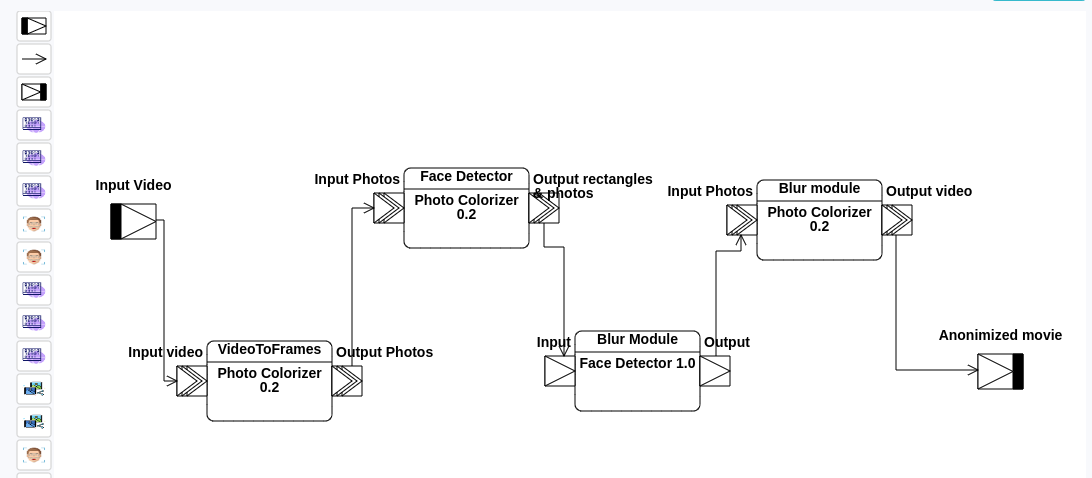
\includegraphics[width=0.77\linewidth]{./images/balticlsc-example-diagram.png}
	\caption{Przykładowy diagram przedstawiający aplikację obliczeniową w
		\BalticLSC{}}\label{rys:przykladowy-diagram-balticlsc}
\end{figure}

Istniejący edytor diagramów w \BalticLSC{} dostępny jest jako część aplikacji
przeglądarkowej udostępnionej przez platformę. Do komunikacji z aplikacją
serwerową wykorzystuje inną reprezentację aplikacji obliczeniowej --- zapisuje
ją w postaci pudełek (prostokątów) oraz połączeń między nimi. Nie komunikuje
się on z aplikacją serwerową przesyłając informacje o strukturze modelu
zgodnej z metamodelem języka \CAL{}. Sprawia to, że po obu stronach (serwera
i aplikacji przeglądarkowej) potrzebne są dodatkowe transformacje
przetwarzające ogólny opis diagramu na model aplikacji obliczeniowej.

\SiriusWeb{}~\cite{sirius-web-github} jest narzędziem przygotowywanym przez
firmę \emph{Eclipse} do tworzenia edytorów
diagramów działających w przeglądarce bazujących na metamodelach w formacie
\Ecore{} w ramach technologii \EMF{}.
Jest ona wykorzystywana od~roku
2007~\cite{eclipse-sirius-wikipedia}, a metamodele
w~przeszłości mogły być tworzone używając oprogramowania \SiriusDesktop{}.
Wykorzystując \SiriusWeb{} można w prosty sposób otrzymać aplikację
przeglądarkową umożliwiającą możliwości przeglądania i edycji modeli zbliżone
do tych,
które dotychczas oferowała jedynie aplikacja wymagająca instalacji na
komputerze użytkownika. Oprócz łatwiejszego dostępu do edytora diagramów dla
nowych użytkowników, wykorzystanie technologii przeglądarkowych do budowy
edytora diagramów pozwala na dodanie mechanizmów kontroli dostępu do
wybranych modeli dla pewnych użytkowników, a także możliwości współpracy nad
modelem przez różne osoby w~czasie rzeczywistym.

W ustrukturyzowanym modelu zawierającym obiekty dziedzinowe w nietrudny sposób
można wyrazić reguły determinujące poprawność semantyczną modelu.
\SiriusDesktop{} pozwala w~tym~zakresie na definiowanie semantycznych reguł
walidacyjnych, które są uruchamiane po każdej modyfikacji modelu i pokazują
błędnie umieszczone elementy. Odpowiednik tej~funkcjonalności jest pożądany
także w edytorach diagramów opartych na \SiriusWeb{}.

W ramach tej pracy magisterskiej przygotowany został edytor diagramów dla
systemu \BalticLSC{} korzystający z \SiriusWeb{}. Edytor ten bazuje na
formalnym metamodelu w formacie \Ecore{} opisującym język \CAL{} do
opisu aplikacji obliczeniowej. Ponadto, dostarczona została metoda sprawdzania
poprawności przygotowywanych przez użytkownika modeli na podstawie
zdefiniowanych reguł walidacji.

\section{Motywacja i cel pracy}

Jedną z alternatyw do wykorzystania \SiriusWeb{} do budowy edytora diagramów
jest
wykorzystanie gotowych bibliotek \JavaScript{} do wyświetlania i modyfikacji
diagramów (przykłady: \emph{react-diagrams}~\cite{react-diagrams-github},
\emph{Cytoscape.js}~\cite{cytoscape-js-homepage},
\emph{vis-network}~\cite{vis-network-github}). Są one ogólnymi narzędziami
pozwalającymi na zbudowanie własnego edytora diagramów. Dają sporą dowolność w
kwestii wyświetlania diagramu oraz
dostępnych funkcjonalności. Nie narzucają one
wykorzystania ustrukturyzowanych modeli poprzez wymaganie stworzenia
metamodelu. Z uwagi na swoją ogólność są trudniejsze do dostosowania do
własnych potrzeb, ponieważ funkcjonalności takie jak zapisywanie modeli w bazie
danych, współpraca w czasie rzeczywistym, walidacja modelu należy
zaimplementować samemu. Ponadto, modyfikacja takiego edytora diagramów wymaga
znajomości języka \JavaScript{}.

\SiriusWeb{} dostarcza większość z tych
funkcjonalności wymagając jedynie wskazania metamodelu, który ma wykorzystywać.
Korzyści płynące z łatwego do przygotowania przeglądarkowego edytora diagramów
dla wybranych przez
nas modeli prezentują technologię \SiriusWeb{} jako interesującą i wartą
użycia,
pomimo jej wczesnej fazy rozwoju i braku dokumentacji.

Celem tej pracy magisterskiej jest zbadanie możliwości udostępnianych przez
\SiriusWeb{} poprzez wykorzystanie go do przygotowania edytora
diagramów dla modeli języka \CAL{}~na~platformie \BalticLSC{}. Elementem
edytora,
na który należy zwrócić szczególną uwagę, jest możliwość walidacji modeli,
czyli weryfikacji ich~poprawności strukturalnej i semantycznej.

Ponadto, praca ta będzie jednym z pierwszych zastosowań \SiriusWeb{} wykonanych
przez osoby spoza zespołu budującego tą technologię, co może dostarczyć
dodatkowych informacji zwrotnych na temat prostoty jego wykorzystania, a także
napotkanych błędów i~niedociągnięć. Dla osób rozważających budowę edytora
modeli w oparciu o \SiriusWeb{}, praca ta będzie stanowiła źródło informacji o
wrażeniach z wykorzystania tej technologii, co pomoże podjąć bardziej świadomą
decyzję o używanych technologiach.
Z uwagi na brak dostępnej dokumentacji \SiriusWeb{}, praca ta może służyć
również jako przykład wykorzystania własnego metamodelu w tym edytorze
diagramów.

Taki edytor diagramów bazujący na \SiriusWeb{} mógłby również zostać
wykorzystany
w~aplikacji przeglądarkowej platformy \BalticLSC{}. Jest on oparty o
ustrukturyzowany opis modelu, co pozwoliłoby na uproszczenie metody komunikacji
między serwerem aplikacyjnym a~aplikacją przeglądarkową, ponieważ nie byłyby
wymagane transformacje z aktualnego, ogólnego formatu danych do formatu
zgodnego z metamodelem.

\section{Zakres pracy}

W ramach pracy magisterskiej wykonano następujące czynności:

\begin{itemize}
	\item Stworzenie metamodelu języka \CAL{} w formacie \Ecore{} z
	      wykorzystaniem \SiriusDesktop{}.
	\item Wykorzystanie tego metamodelu w \SiriusWeb{}. Zgłoszenie usterek
	      autorom \SiriusWeb{} poprzez \GitHub{}.
	\item Porównanie możliwości \SiriusWeb{} i \SiriusDesktop{}. Zgłoszenie
	      brakujących funkcjonalności autorom \SiriusWeb{} poprzez
	      \GitHub{}.
	\item Dodanie do metamodelu elementów usprawniających pracę z nim
	      (automatyzacja niektórych czynności, dodanie ograniczeń
	      utrudniających
	      zrobienie błędu).
	\item Modyfikacja przeglądarkowego interfejsu użytkownika \SiriusWeb{}
	      poprzez dodanie do~niego przybornika z \BalticLSC{}. Przybornik
	      umożliwia w
	      łatwy sposób dodanie nowych elementów do modelu.
	\item Dodanie mechanizmu walidacji semantycznej modelu sprawdzającego
	      poprawność modelu z regułami zdefiniowanymi w języku \Java{}.
	\item Stworzenie planu integracji rozwiązania z \BalticLSC{}.
	\item Stworzenie przykładowej aplikacji przeglądarkowej zawierającej
	      jedynie edytor diagramów z \SiriusWeb{}. Taki przykład pokazuje
	      możliwość
	      wykorzystania \SiriusWeb{} jako element innej aplikacji
	      przeglądarkowej.
\end{itemize}

\vspace{1em}

\noindent Poza zakresem pracy pozostały następujące czynności:

\begin{itemize}
	\item Integracja stworzonego rozwiązania jako alternatywnego edytora
	      diagramów dla systemu \BalticLSC{}.
	\item Naprawa zgłoszonych usterek w \SiriusWeb{}.
\end{itemize}


\chapter{Nienudny tytuł dla teorii}
Można też pisać wszystko w jednym pliku, tak jak przyzwyczajają do tego gorsze programy, ale wtedy główny plik będzie bardzo duży i trudniejszy w zarządzaniu.
% fragment nieużywany albo jeszcze niedodany można zakomentować
%\input{tekst/teoria}
%\input{tekst/donapisania}

\chapter{Niebanalny tytuł kolejnego rozdziału}
Test ciągłości numeracji po przejściu do nowego rozdziału.


\begin{figure}[!hb]
	\centering 
\includegraphics[width=0.618\linewidth]{Kopernik.jpg}
	\caption{Powtórzony rysunek dla testu ciągłości numeracji}
	\label{rys:kopernik2}
\end{figure}

\begin{table}[!b]
 \centering
  \begin{tabular}{p{2.5cm}c|l}
    Data        &   Godzina (UTC)   &   Zdarzenie\\\hline
    2016-05-09  &   14:57           &   Tranzyt Merkurego\\\hline
    2017-08-11 --~2017-08-13  & --- &   Maksimum Perseidów \\\hline
    2018-07-27  &   20:22           &   Całkowite zaćmienie Księżyca\\\hline
    2019-08-24  &   17:04           &   Koniunkcja Wenus i Mars w odległości - 0°17`\\\hline
    2020-12-21  &   16:00           &   Koniunkcja Jowisz i Saturn w odległości 0°06`
  \end{tabular}
 \caption{\label{tab:zjawiska2}Powtórzona tabelka dla testu ciągłości numeracji}
\end{table}

\begin{equation}
    \frac{\partial^2 y}{\partial x^2} = \frac{\mu}{F} \; \frac{\partial^2 y}{\partial t^2}
\end{equation}

\begin{lstlisting}[language=Python,
    caption={Powtórzony kod dla testu ciągłości numeracji},
    label={lst:hello2}]
#!/usr/bin/env python
# -*- coding: utf-8 -*-
"""Simple world of hello.
"""

import sys

def main():
    """The one and only function"""
    fib = lambda n: reduce(lambda x, n: [x[1], x[0]+x[1]], range(n), [0, 1])[0]
    try:
        print(fib(int(sys.argv[1])))
    except:
        print("Hello World!")

if __name__ == "__main__":
    main()
\end{lstlisting}


% Przykładowy wypełniacz
\lipsum{21-40}


\chapter{Podsumowanie}
\chapter{Podsumowanie}

W tym rozdziale zostaną opisane wyniki pracy magisterskiej oraz wnioski z niej
wyciągnięte, a także możliwości na jej dalszy rozwój przygotowanego
rozwiązania.

\section{Wyniki pracy}

W ramach tej pracy magisterskiej technologia \emph{Sirius Web} została
wykorzystana do stworzenia edytora diagramów opisujących aplikacje obliczeniowe
systemu \emph{BalticLSC}. Wykorzystuje on przygotowany specjalnie w tym celu
metamodel \gls{EMF} języka \gls{CAL}. Do edytora zostały dodane narzędzia i
funkcjonalności pomagające w efektywniejszym i szybszym tworzeniu modeli.
Ocenione zostały także możliwości edytora i porównane z możliwościami
konkurencyjnej poprzedniej wersji edytora bazującego na metamodelach \gls{EMF},
czyli \emph{Sirius Desktop}.

Edytor użyty jest domyślnie jako część interfejsu przykładowej aplikacji
wykorzystującej bibliotekę \emph{React}.
Jako jedna z części tej pracy udostępniono interfejs programistyczny
pozwalający na wyświetlenie edytora w dowolnej aplikacji przeglądarkowej
wykorzystując wyłącznie funkcje w języku \emph{JavaScript}, bez wymogu używania
konkretnej biblioteki.
Pozwala to na wykorzystanie go jako
alternatywny edytor diagramów platformy \emph{BalticLSC}, która wykorzystuje
bibliotekę \emph{Vue.js}. Zostało to
zademonstrowane poprzez przygotowanie aplikacji przeglądarkowej wyświetlającej
edytor diagramów jako część swojego interfejsu.

Edytor domyślnie pozwala na wyświetlenie modeli w formie diagramów zgodnie z
definicją reprezentacji z metamodelu \gls{EMF} oraz na podstawowe możliwości
edycji tych modeli. Zachowana jest funkcjonalność interpretacji języka
\gls{AQL} do wyrażenia bardziej zaawansowanej logiki czy wyrażeń opisujących
właściwości metamodelu. Jednak nie wszystkie mozliwości metamodeli \gls{EMF}
wspierane przez \emph{Sirius Desktop} są obsługiwane przez \emph{Sirius Web}.
Niektóre elementy są również inaczej wyświetlane co sprawia, że metamodel
należy szczególnie dostosować pod \emph{Sirius Web}.

Różnice między \emph{Sirius Web} i \emph{Sirius Desktop}, a także błędy w
funkcjonowaniu oraz brakujące funkcjonalności edytora sprawiły, że autorom
projektu zostało zgłoszone 20 usterek w repozytorium projektu
\texttt{sirius-components} na platformie \emph{GitHub}. Dwie z nich zostały
rozwiązane podczas pisania pracy magisterskiej. Część problemów posiadała
alternatywne rozwiązania, które pomimo swoich wad pozwalały uzyskać zamierzony
efekt. W innych przypadkach brakujące funkcjonalności należało zaimplementować
samemu.

Funkcjonalnościami dodanymi do edytora w ramach pracy magisterskiej są
mechanizm walidacji semantycznej modeli języka \gls{CAL} oraz implementacja
przybornika wyświetlającego listę dostępnych modułów aplikacyjnych z platformy
\emph{BalticLSC}. Modyfikacja kodu serwera aplikacyjnego zazwyczaj była
łatwiejsza od modyfikacji kodu aplikacji przeglądarkowej, ponieważ dzięki
mechanizmowi wstrzykiwania zależności z platformy \emph{Java Spring}
często wystarczyło jedynie dodać nowe klasy i ewentualnie zmienić kilka linii w
już istniejących.

Zmiana kodu interfejsu użytkownika aplikacji przeglądarkowej była pracochłonna
i wiązała się ze skopiowaniem kodu źródłowego tych komponentów, które mają być
modyfikowane. \emph{Sirius Web} nie udostępnia prostych metod na dodanie
własnych elementów interfejsu do istniejących komponentów, więc kopiowanie i
edycja ich kodu źródłowego jest jedynym rozwiązaniem. Dodaje to natomiast pracy
przy późniejszych aktualizacjach do nowej wersji ponieważ należy upewnić się
czy kod skopiowanych komponentów został zmieniony. Jeżeli tak, należy odtworzyć
te zmiany, ponieważ w przeciwnym wypadku aplikacja może działać niepoprawnie.

Wykorzystanie, a później modyfikacja edytora \emph{Sirius Web} była utrudniona
przez brak dokumentacji, niewielką liczbę publicznie dostępnych przykładów
wykorzystania rozwiązania oraz małą liczbę użytkowników zadających pytania,
których odpowiedzi byłyby widoczne publicznie. Te wszystkie aspekty wynikają z
krótkiego czasu życia projektu, ponieważ został on rozpoczęty w 2018 roku, a
dopiero w 2020 roku jego kod źródłowy został udostępniony na platformie
\emph{GitHub}. Praca nad edytorem wymagała poświęcenia sporej ilości czasu na
zrozumienie jak \emph{Sirius Web} działa poprzez czytanie kodu źródłowego
przykładowej aplikacji z repozytorium \texttt{sirius-web}, jak i poszczególnych
klas biblioteki z repozytorium \texttt{sirius-components}. Gdy znalezienie
odpowiedzi na nurtujące pytania zajmowało zbyt dużo czasu, zadawano pytanie
autorom projektu za pomocą \emph{GitHub Issues}.

Umożliwienie edycji modeli w przeglądarce ma sporo zalet w porównaniu do
edytorów funkcjonujących jako aplikacje natywne, takie jak \emph{Sirius
	Desktop}. Nie wymaga on procesu instalacji, można szybciej udostępnić
model innym użytkownikom, łatwiej jest przeprowadzać aktualizację metamodelu do
nowszej wersji, zmiany w modelach są automatycznie propagowane do wszystkich
użytkowników w czasie rzeczywistym. Sam interfejs został też odświeżony i
wygląda bardziej estetycznie w porównaniu do \emph{Sirius Desktop}.

Wykorzystanie sieci Internet do obsługi edytora ma też swoje wady. Niektóre z
nich są szczególnie problematyczne i widoczne z uwagi na przyjęty schemat
komunikacji między aplikacją przeglądarkową a serwerem aplikacyjnym. Na wolnych
lub niestabilnych łączach edytor może działać Wykorzystanie sieci Internet do
obsługi edytora ma też swoje wady. Niektóre z nich są szczególnie
problematyczne i widoczne z uwagi na przyjęty schemat komunikacji między
aplikacją przeglądarkową a serwerem aplikacyjnym. Na wolnych lub niestabilnych
łączach edytor może działać Wykorzystanie sieci Internet do obsługi edytora ma
też swoje wady. Niektóre z nich są szczególnie problematyczne i widoczne z
uwagi na przyjęty schemat komunikacji między aplikacją przeglądarkową a
serwerem aplikacyjnym. Na wolnych lub niestabilnych łączach aplikacja edytor
może działać ze sporym opóźnieniem i powodować frustrację podczas jego obsługi,
bo każda zmiana modelu musi zostać wprowadzona przez serwer aplikacyjny.
Problem pogarsza fakt, że przy każdej zmianie wysyłane są wszystkie informacje
o modelu zamiast jedynie informacji o zmienionych fragmentach.

Centralizacja przechowywania modeli w obrębie serwera aplikacyjnego często
oznacza, że pożądaną funkcjonalnością jest kontrola dostępu użytkowników do
modeli. W organizacjach użytkownicy powinni mieć ograniczony dostęp do zasobów
i być uwierzytelnieni. \emph{Sirius Web} domyślnie nie ma żadnych ograniczeń
dostępu do modeli, jednak większość operacji można zabezpieczyć za pomocą
rozwiązania \emph{Spring Security}. Jedyny kanał, który nie może zostać
zabezpieczony, są subskrypcje \emph{GraphQL}, które wymagają specjalnej metody
uwierzytelnienia. Za ich pomocą dowolna osoba może otrzymać informacje o
zawartości dowolnego modelu. Jest to poważna wada, ponieważ nie można wtedy
zapewnić kontroli dostępu, co jest podstawowym wymaganiem w aplikacjach
wykorzystywanych w organizacjach. Prawdopodobnie skreśla to \emph{Sirius Web}
jako możliwe rozwiązanie chyba, że wdrożone są dodatkowe mechanizmy
bezpieczeństwa niemożliwiające dostępu do serwera aplikacyjnego osobom
nieuwierzytelnionym.

Projekt \emph{Sirius Web} jest aktywnie rozwijany. W ciągu miesiąca (od 15
grudnia 2021 r.\ do 15 stycznia 2022 r.) zostało wydanych 9 nowych wersji tego
oprogramowania. Niektóre z nich wymagały jedynie pobrania nowych plików
źródłowych, a inne z nich wprowadzały zmiany łamiące kompatybilność wsteczną i
wymagające niekiedy znacznych zmian w kodzie źródłowym. Zmiany te były najpierw
wprowadzane przez zespół pracujący nad tą technologią w repozytorium
\texttt{sirius-web}, więc można było je wykorzystać podczas aktualizacji
własnej kopii edytora. Było to natomiast tym trudniejsze, im bardziej edytor
został przez nas zmodyfikowany, ponieważ wtedy kod bardziej się róznił i
narzędzia umożliwiające automatyczne wprowadzanie zmian (pochodzące z systemu
kontroli wersji \emph{git}) nie wiedziały jak je wprowadzić.

Podsumowując, wszystkie zamierzone cele pracy magisterskiej zostały osiągnięte.

\section{Wnioski}

\emph{Sirius Web} jest technologią eksperymentalną, nieposiadającą jeszcze
dokumentacji ani wielu przykładów zastosowania. Brakuje też listy
nieobsługiwanych funkcjonalności w porównaniu do \emph{Sirius Desktop}. Praca z
tego typu projektem wprowadza ryzyko, ponieważ trudniej oszacować czas
i wysiłek potrzebny na jego wykorzystanie czy wdrożenie nowych funkcjonalności.
Niektóre proste z pozoru dodatki mogą okazać się nietrywialne z uwagi na sposób
działania rozwiązania.

Kolejnym ryzykiem, które należy brać pod uwagę szczególnie wykorzystując nowe
technologie jest możliwość znalezienia usterek, które będą wymagały czasu na
ich naprawienie. Większość z problemów zgłoszonych w projekcie \emph{Sirius
	Web}
nie zostało naprawionych pomimo, że od ich zgłoszenia minęły w niektórych
przypadkach nawet 3 miesiące. Planując projekt warto uwzględnić na jego samym
początku czas na sprawdzenie możliwości wykorzystywanych narzędzi i w przypadku
niepewności przygotować przykład ich zastosowania, który pomógłby w
znalezieniu problemów lub brakujących funkcjonalności na wczesnym etapie
projektu. W ten sposób można wcześniej zmienić harmonogram projektu i podjąć
działania minimalizujące negatywne efekty, jak na przykład przeznaczenie
większej ilości czasu na naprawę usterek albo całkowita rezygnacja z niektórych
funkcjonalności.

Rozpoczynając pracę z nowymi technologiami warto najpierw poznać podstawy ich
działania, a dopiero później próbować je w znaczącym stopniu zmodyfikować.
Warto także najpierw spróbować wykorzystać je osobno zanim spróbuje się je
zintegrować ze sobą. Tak było z \emph{Java Spring}, \emph{Maven} oraz
\gls{EMF}, z którymi autor pracy nie miał wcześniej doświadczenia. Próby
modyfikacji bez znajomości zasad działania tych technologii prowadziły do
błędów, często trudnych do zrozumienia, oraz frustracji. Spędzenie kilku godzin
na poznawaniu tych technologii i wykorzystaniu ich w izolacji przed
modyfikowaniem \emph{Sirius Web} używającego ich wszystkich sprawiło, że
szybciej wykonano postępy.

Mając do czynienia z dwoma podobnymi technologiami korzystającymi z tego samego
źródła trzeba mieć na uwadze możliwe niekompatybilności. Aby je zweryfikować
należy wykorzystać je zaczynając od tych najprostszych, zanim przejdzie się do
bardziej skomplikowanych. Pozwoli to zaoszczędzić czas spędzony na
dostosowywaniu jednego z rozwiązań podczas gdy drugie nie będzie w stanie
obsłużyć tych samych funkcjonalności. Tak było w przypadku wsparcia różnych
składników metamodeli \gls{EMF} przez \emph{Sirius Desktop} i \emph{Sirius
	Web}. Najpierw zainwestowano czas w przygotowywanie kompletnego
metamodelu z
wykorzystaniem \emph{Sirius Desktop}, po czym okazało się, że część z
funkcjonalności nie jest wspierana przez \emph{Sirius Web} lub jest wspierana
częściowo i metamodel wymaga zmian. Zmarnowano w ten sposób czas na
przygotowywanie elementów, które ostatecznie nie były potrzebne, ponieważ celem
pracy było wykorzystanie metamodelu wyłącznie w \emph{Sirius Web}.

Wykorzystanie technologii \emph{Docker}~\cite{wikipedia-docker} znacznie
ułatwia rozpoczęcie pracy z
nowymi narzędziami oraz wdrożenie projektu wewnątrz maszyny wirtualnej.
Stworzenie obrazu \emph{Docker} zawierającego serwer aplikacyjny \emph{Sirius
	Web} umożliwiło dużo szybsze wdrożenie aplikacji oraz jej aktualizację
do nowej
wersji, ponieważ wystarczyło zainstalować silnik \emph{Docker}, a później
pobrać i uruchomić obraz. Nie było wymagane instalowanie środowiska \emph{Java}
wewnątrz maszyny wirtualnej. Nie występowały też błędy związane z
kompatybilnością czy brakiem narzędzi zainstalowanych na jednym ze środowisk.
Warto rozważyć technologię \emph{Docker} w projektach, aby ułatwić ich
wdrożenie.

\section{Możliwości na rozwój}

Wymienić co można zrobić dalej:

\begin{itemize}
	\item integracja z BalticLSC
	\item dodanie większej liczby reguł walidacji semantycznej
\end{itemize}

